\subsection{Challenges along with the transition}

\begin{figure*}[htbp!]
	\centering
	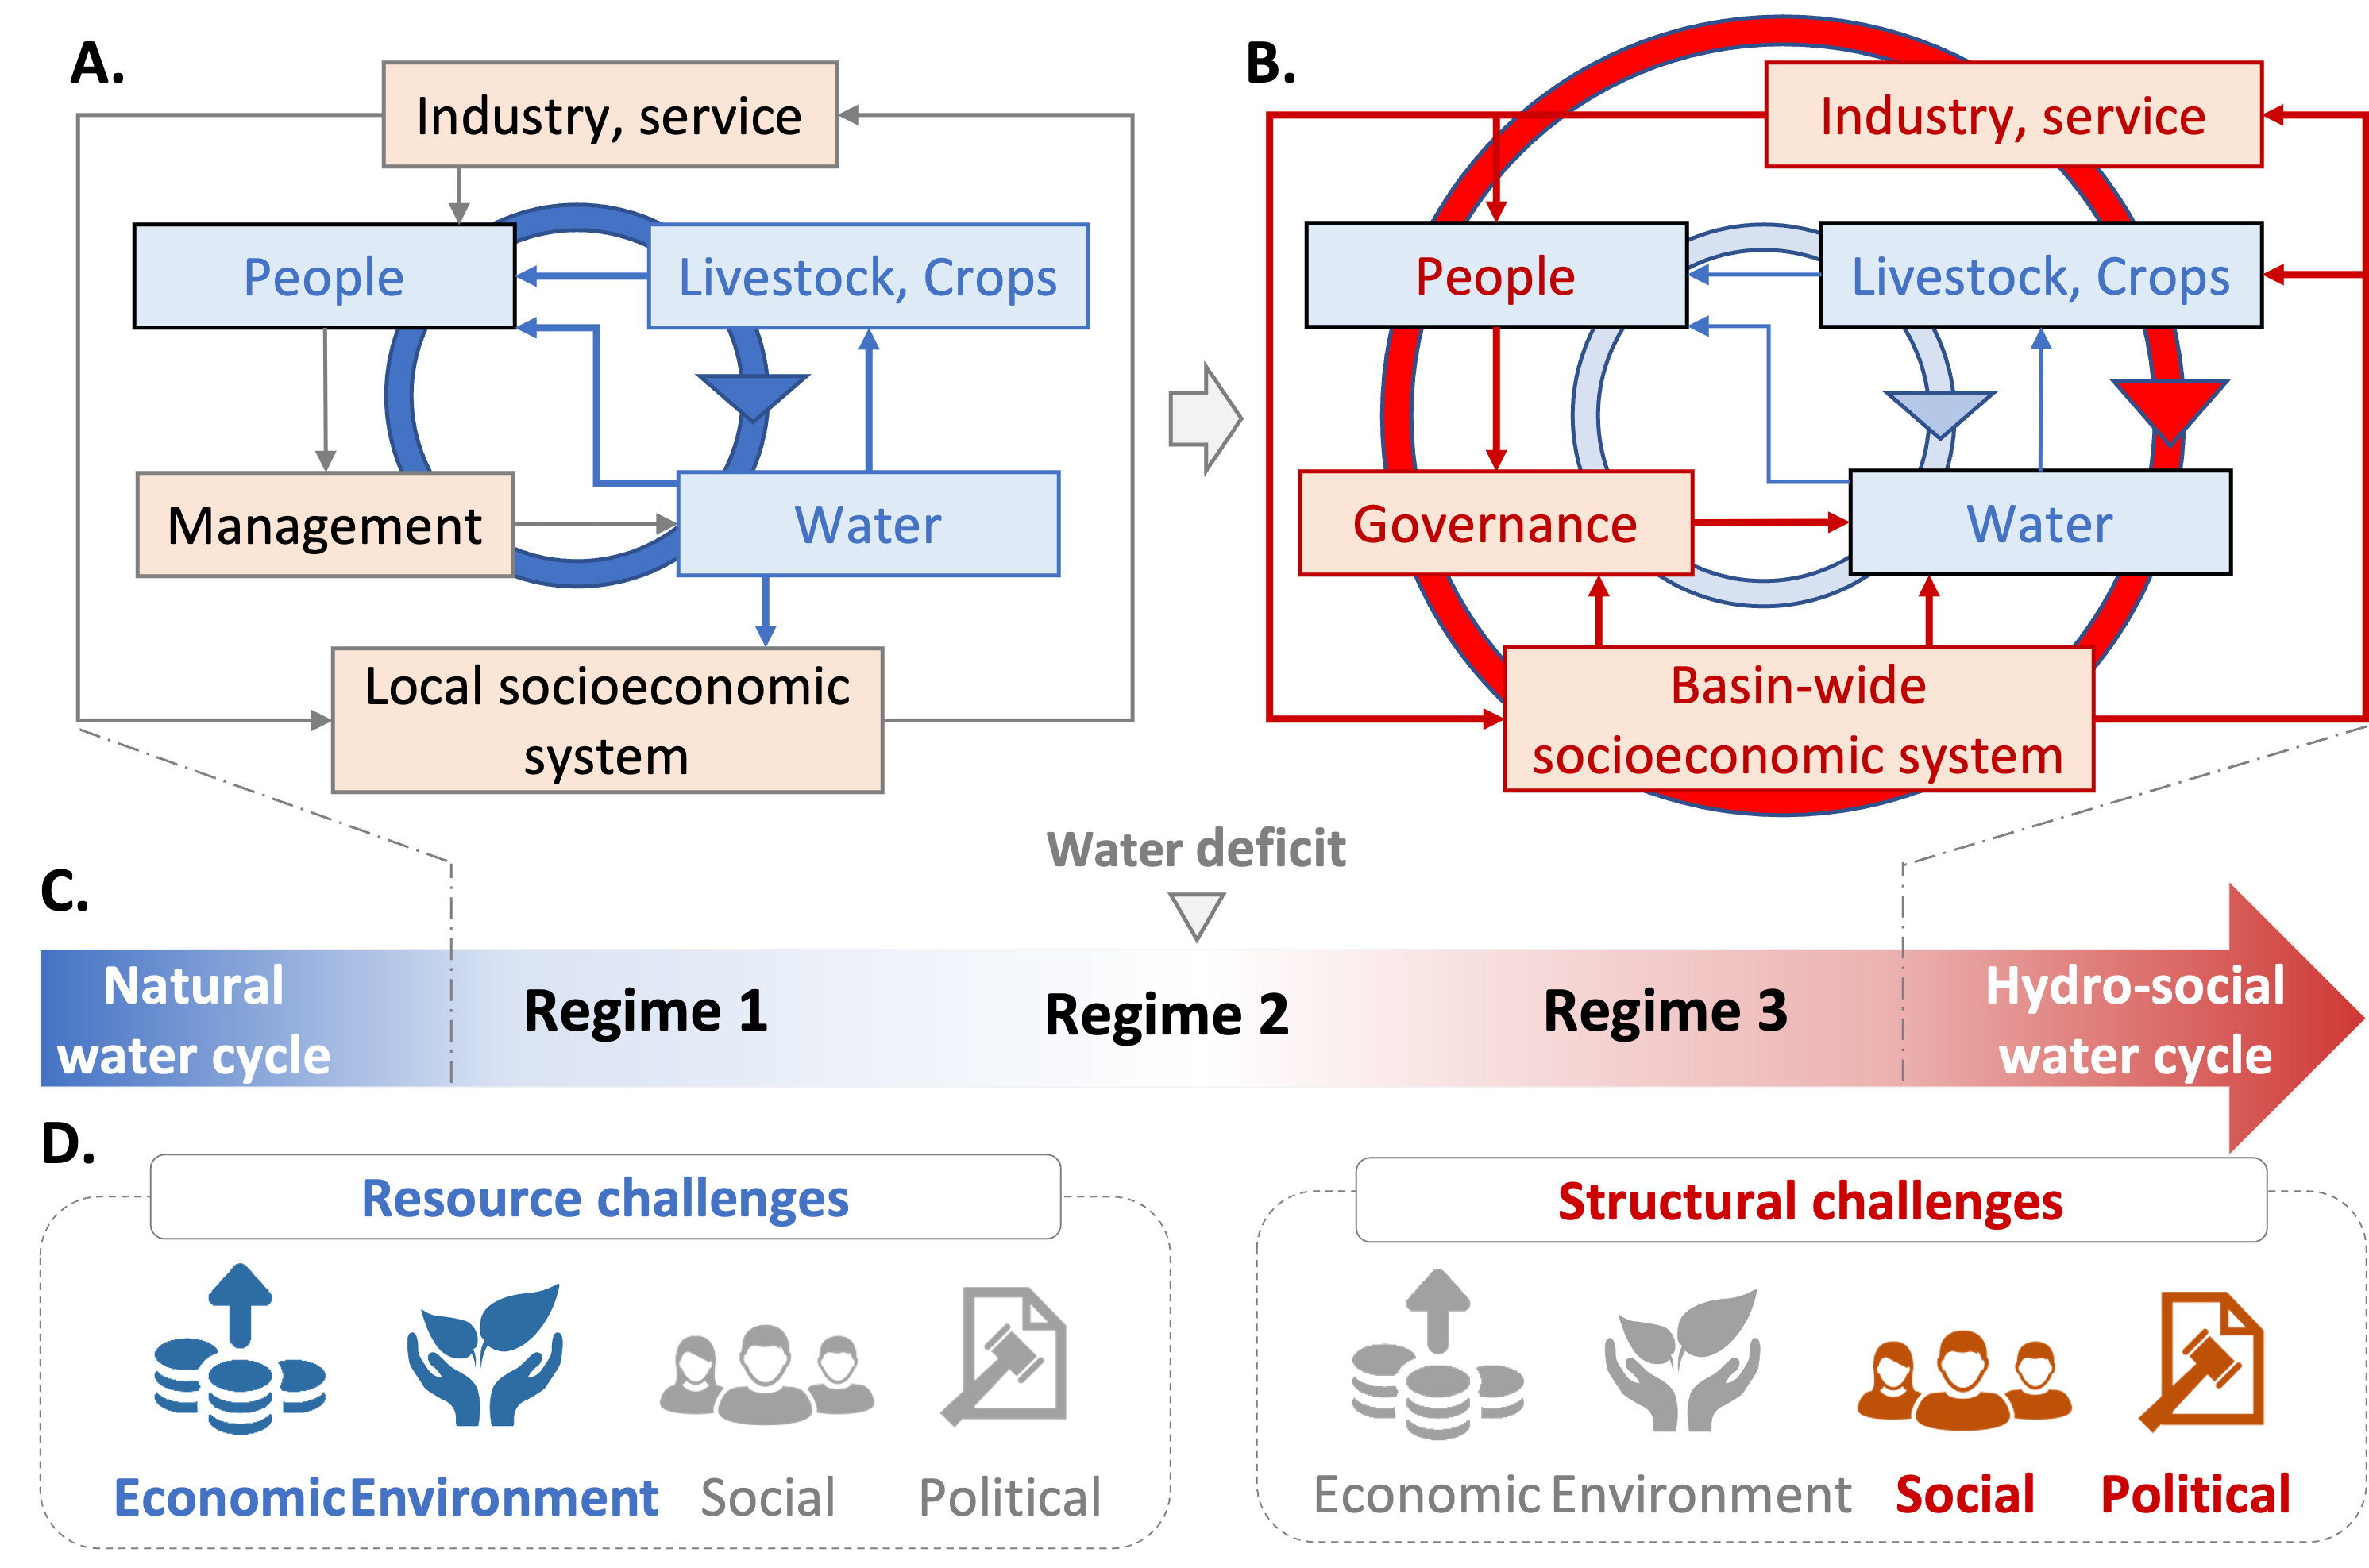
\includegraphics[width=0.9\linewidth]{main/transition.png}
	\caption{
		Transition schema in hydrosocial cycle and water governance regimes. The natural water cycle dominates blue pathways while socio-economic feedback dominate red pathways.
		\textbf{A. Early phase.} As socio-economic systems developing, non-provisioning water demand increases; simultaneously, increased adaptive capacity by engineering allows people to manage water resources for alleviating the water stress.
		\textbf{B. Late phase} With further human interventions, trade-offs between provisioning-purpose and non-provisioning water use become prominent; basin-wide socio-economic system requires to more organized water governance.
		%! The note to C. makes no sense! from the refree 2.
		Thus, \textbf{C. the hydrosocial water cycle transition} correlates with the water governance regime shifts (in the YRB, they are identified as massive supply regime, transformation governance regime, and adaptation oriented regime). The transformation governance regime shift occurs following water deficit, with rapid growth of adaptive capacity.
		\textbf{D. Water governance challenges} Through the transitional regimes, water governance faces primarily economic and environmental challenges in the early phase and social and policy challenges in the late phase.
	}
	\label{fig:summary}
\end{figure*}

% 我们为的研究结果表明,黄河流域能被识别为三个明显的稳态。
Our results show that there have been three distinct but sequential governance regimes within the YRB: a massive supply regime (P1: 1965-1978), a governance transforming regime (P2: 1979-2001) and an adaptation oriented regime (P3: 2002-2013).
Furthermore, shifts between these regimes were caused by different environmental, economic, social or political drivers, deciding who gets water, when and how.
The process echoes how social systems can change water governance regimes by enhancing their adaptive capacity. %! citation
However, the IWGI quantitatively identifies and reveals that abstract pattern, thus characterizing the transition of water governance in detail for the first time.
It is important to note that each indicator or cause changes gradually, but emerging regime shifts move water governance along with the hydrosocial water cycle at a basin scale.
As a result, the water governance challenges were primarily economic and environmental at the beginning of the trajectory and social and policy-related towards the end (Figure~\ref{fig:summary} C and D).

% 在水资源压力较低的大规模供应制度(长江流域1965-1978年)期间,水治理实践倾向于通过建设水库和渠道来增加服务用水(当时主要是供应目的——牲畜和农作物)。
During the massive supply regime with lower water stress (1965-1978 in the YRB), water governance thus tended to boost water supply for services (mainly provisioning purposes then -livestock and crops) by constructing reservoirs and channels.
% 然而,正如“人类将征服自然”的流行口号所暗示的那样,水供应的增加很少考虑到人水关系不可逆转的变化,从而也急剧增加了水的需求,很少考虑到流域的保护。
As the popular slogan ``man will conquer nature'' suggested, however, the enhancement of water supply aligned with little consideration of the irreversible changes in the human-water relationship, thus drastically increasing water demand with little consideration in basinal conservation.
\cite{zhouDecelerationChinahuman2020}.
% 在那十年里,灌溉农田和引水设施的迅速扩张,使负担过重的长江水利枢纽接近临界点,在这个临界点上,持续增加供应来满足无限的需求是不现实的
The rapid expansion of irrigated farmland and water diversion facilities in that decade brought the overburdened YRB close to the critical point, where keeping increasing supply to meet the unlimited demand is unpractical
% 结果,自1972年以来,超过80%的地表水使用量导致了河流的频繁枯竭,随之而来的是生态问题,如湿地的萎缩和生物多样性的下降。
As a result, the over 80\% surface water use then led to river depletions frequently since 1972, with ecological issues, such as wetlands shrinkage and declines in biodiversity.
% 此外,由于处于上升阶段的工业经济也受到水资源压力的限制,现有的水治理模式严重导致了巨大的社会-生态危机和对可持续性的重大挑战
In addition, as the water stress also limited the industrial economy in the ascendant, the existing modes of water governance led to a social-ecological crisis and challenged sustainability rigorously
\cite{wohlfartRiverBasinCourse2016}.

The start of the governance transforming regime (P2: 1979-2001) coincided with the rising competition for water use after the ``reform and opening-up''.
% 正如理论预测的那样
The results in the YRB keep in line with the suggestions from the theoretical analysis: continuous increases in water demand when the basinal total supply is stable can follow substantial changes in governance regime and the rapid enhancement in overall social adaptive capacity %! Citation.
% 作为制度转变的先行者
Being a pioneer in shifting governing institutions, the YRB triggered a series of changes in ``who gets water, when and how'' during this regime: slowing growth of irrigated acreage; leading water-saving infrastructure; China's first water quota scheme; The preliminary cross-boundaries water transfer plan and so on
\cite{wangThirtyYearsYellow2018}.
% 因此,1999年黄河的最后一次枯竭
Consequently, though water stress remained and increased (mainly led by reducing streamflow and flexibility), the last depletion of the Yellow River in 1999 added a footnote to the climax of this transformation in water governance.

Finally, it came into an adaptation-oriented regime (P3: 2002-2013), when drastically shifting in societies occurred with stable water stress.
Socio-economic trade-offs between water-dependent regions and sectors played a more important role in this regime, so water governance had to achieve efficient water allocation while balancing different purposes in the face of limited water supply
\cite{dalinBalancingwaterresource2015}.
Reconstruction of resources widespread in different industries and regions was calling for adaptation in water governance, where the urgent requirements of adjusting the rigid quota shares from the previous regime can be an example.
% 类似的,此稳态下国家层面的水治理政策都在进行补充或调整,因为这种制度的缺失和社会的不公平正成为流域新的治理挑战。
Like this, many national-level governing practices were proposed under the regime because the absence of such policies with the social dilemma of high-quality development became new structural challenges for water governance
\cite{konarExpandingScopeFoundation2019}.

% 一般来说,在向水社会循环的转变过程中,三种治理制度之间的转变是依次发生的。
In general, the shift between the governance regimes advances in parallel with the trajectory of the hydrosocial cycle (Figure~\ref{fig:summary}A, B and C).
The transition from biophysical control to social and institutional control of ecosystem dynamics may become increasingly widespread in social-ecological systems as increasing anthropogenic impacts gradually change the world
\cite{bestPaceHumanInducedChange2020,cummingLinkingeconomicgrowth2018,cummingImplicationsagriculturaltransitions2014}.
With intensive anthropogenic intervention, the YRB may be the most prominent example in this general transition of water governance -``improving supply, transforming governance, and enhancing adaptation'' %! Citation.
The transition regimes identified here also echo the two kinds of major water governance challenges globally (resource challenges and structural challenges, Figure~\ref{fig:summary} and \textit{SI Appendix} Fig. S9)
\cite{singhWaterGovernanceChallenges2019,porcherFacingChallengesWater2019}.
Our analysis suggests that the early phase of transition often leads to resource-focused challenges that result from economic and environmental change, while structural challenges dominate the later phases of governance in social and political aspects.
Resource challenges, represented as water shortage and water supplying difficulties, are mainly faced by undeveloped and developing basins
\cite{allanNavigatingcomplexitiescoordinated2019,florkeWatercompetitioncities2018,liuWaterSustainabilityChina2012}.
Alternatively, highly-controlled and developed basins (especially for transboundary rivers) must mainly resolve structural challenges, such as water disputes or lack of equity, and maybe in urgent need of novel flexible, efficient sociopolitical governance structures %! Kitroeff citation wrong
\cite{kitroeffThisWarCrossBorder2020,kitroeffThisWarCrossBorder2020,roobavannanRoleSectoralTransformation2017,unep-dhiTransboundaryRiverBasins2016}.
Typically, resource and structural challenges occur sequentially during the transition of water governance within the YRB.
From the perspective of the core dimensions emphasized by the UNDP for water governance, our proposed schema connects governance challenges and the transformation of large river basins toward a hydrosocial water cycle.

\subsection{Implications, limitations, and future directions}
\label{Outlook}

% Implications
Water governance gradually becomes a national or international concern from a primarily local concern because large river basins are critical sources of ecosystem services, economic development, and human well-being.
As the ubiquitous tele-coupling is rising additional water governance challenges in the tighter connected world, the transition of hydrosocial cycle and regime shifts align with different human-water relationships.
Within the growing hydro-social cycle, the IWGI index depicts the increase of the adaptive capacity and sketches the transitional water governance regimes in a relatively straightforward but comprehensive way.
It is important for scientists and decision-makers to recognize the changing governance challenges because models, institutions, engineering, and approaches developed under one regime are not necessarily useful under a different regime
%! \cite{cummingLinkingEconomicGrowth2018, reyersSocialEcologicalSystemsInsights2018}.
In the case of the YRB, an essential institution of water quota in the governance transforming regime became rigid during the enhanced adaptation phase.
On the contrary, additional water from the ambitious cross-basins water diversion project, which originated in the phase of massive supply, can play an even more crucial role in today's enhancing adaptation phase.
Overall, applications of IWGI can induce a straightforward understanding of the water governance in the transition of the hydrosocial cycle, as descriptions from some previous conceptual frameworks suggested for all large-scale basins worldwide.

%! limitations
One of the main limitations of applying IWGI is abundant data availability for a long-term period.
For example, we used the stress-flexibility-variability (SFV index) here, one of the most comprehensive indexes, as an indicator of the water stress dimension.
With other indicators, therefore, we obtained various datasets in the YRB: water use in different regions and sectors, streamflows in different reaches, reservoir capacity and completion time, with furthermore information in social, economic, and institutional for interpretation.
It means still a gap between the comprehensively identifying and widespread application of IWGI.
However, we assumed that all water governance issues are relative to ``who gets water, when and how'', so water stress, purposes of water services, and water allocation patterns matter.
We suggest that choices of the indicators for the dimensions can be adapted according to available datasets as the intertwines between the underlying components are much more crucial in understanding the transition of governance regimes.

% direction
For today's world, water-related challenges remain one of the major gaps in our progress towards sustainability, while development-first strategies are still a dominant guideline in many places and maybe in opposition to improving governance
\cite{xuAssessingprogresssustainable2020,liuAerosolweakenedsummermonsoons2017,greveGlobalassessmentwater2018}.
% 虽然大多数大型河流流域随着发展而在水管理技术和水利用效率方面有所改善,但淡水利用仍被认为正在接近人类-水系统可能崩溃的行星边界
Although most large river basins have shown improvements in water management technologies and water use efficiency along with development, freshwater use is still approaching planetary boundaries where human-water systems may collapse
\cite{anExploringeffectsGrain2017,degraafEnvironmentalflowlimits2019,hugginssocialecologicaldimensionschanging2020}.
% 我们的分析展示了这种路径的前方很可能是严峻的水治理挑战。
% 总的来说,这种明显的治理失败可能有两个主要原因。
% Overall, there are probably two main reasons for this apparent failure of governance.
% 首先,农业灌溉效率的显著提高通常伴随着灌溉面积的重新扩大,导致水资源压力的趋势不减(效率悖论)
% First, significant improvement in agricultural irrigation efficiency is usually accompanied by a re-expansion of irrigated area, resulting in an unabated trend of water resources stress (the paradox of efficiency)
\cite{graftonparadoxirrigationefficiency2018}.
% 其次,如果没有成功的治理,以水循环为主导的复杂治理结构可能会导致流域尺度上水资源使用的灵活性降低,破坏社会-生态系统的恢复力
In the future, without successful governance, complicated governance structures dominated by hydrosocial water cycles may result in less flexible water use and undermine the resilience of social-ecological systems at a basin-scale
\cite{qinFlexibilityintensityglobal2019,leviaHomogenizationterrestrialwater2020,grillMappingworldfreeflowing2019}.
% 从这些角度来看,我们需要更好、更全面的策略来应对治理挑战,因为核心问题是复杂而难以管理的
From these perspectives, we need more flexible and comprehensive strategies to address governance challenges because the core problems are dynamic and complex
\cite{steffenemergenceevolutionEarth2020,muneepeerakulemergenceresilienceselforganized2020,bodinCollaborativeenvironmentalgovernance2017,biermannNavigatingAnthropoceneImproving2012}.
% 更深入地了解包含非线性变化、制度和过渡思想的治理,应该有助于将治理的重点转移到维持流域社会-生态系统的恢复力和提高其可持续性。
A deeper understanding of governance that incorporates ideas of non-linear change, regimes, and transitions should help to shift the focus of governance towards maintaining the resilience of the basin’s social-ecological system and improving its sustainability.
